\chapter{A Case Study on QO-100 Narrowband Beacon} \label{ch:QO-100}

\section{Ground Station Hardware Architecture} \label{sec:hardware_architecture}

The ground segment for high-rate data acquisition and capture is structured as a sequential RF chain. The architecture is designed to maintain signal integrity from the antenna focal point to the digital processing unit, ensuring that the noise figure is dominated by the LNB’s front-end stage to support the mission's link margin requirements.
\begin{equation*}
    \mathsf{Antenna} \longrightarrow \mathsf{LNB} \longrightarrow \mathsf{Bias\text{-}T} \longrightarrow \mathsf{SDR} \longrightarrow \mathsf{Computer}
\end{equation*}

The first block consists of the radiating system, composed of a parabolic antenna whose feed is mechanically fixed at the primary focus using a rigid four-arm support structure or quadripod . Directly coupled at this focal point is the low-noise block downconverter, or \(\mathsf{LNB}\). The critical function of the \(\mathsf{LNB}\) is to amplify the extremely weak signal received from outer space (around X-band frequencies or $10$~GHz) while injecting the lowest possible amount of thermal noise, and then translate it in frequency using a local oscillator coupled to a significantly lower Intermediate Frequency (\(\mathsf{IF}\)) (typically in L-band, between $1$ and $2$~GHz). This downconversion is essential so that the signal can propagate through an extended-length coaxial cable to the equipment room without suffering severe attenuation or distortion due to high-frequency dielectric losses.

\begin{figure}[htbp]
    \centering
    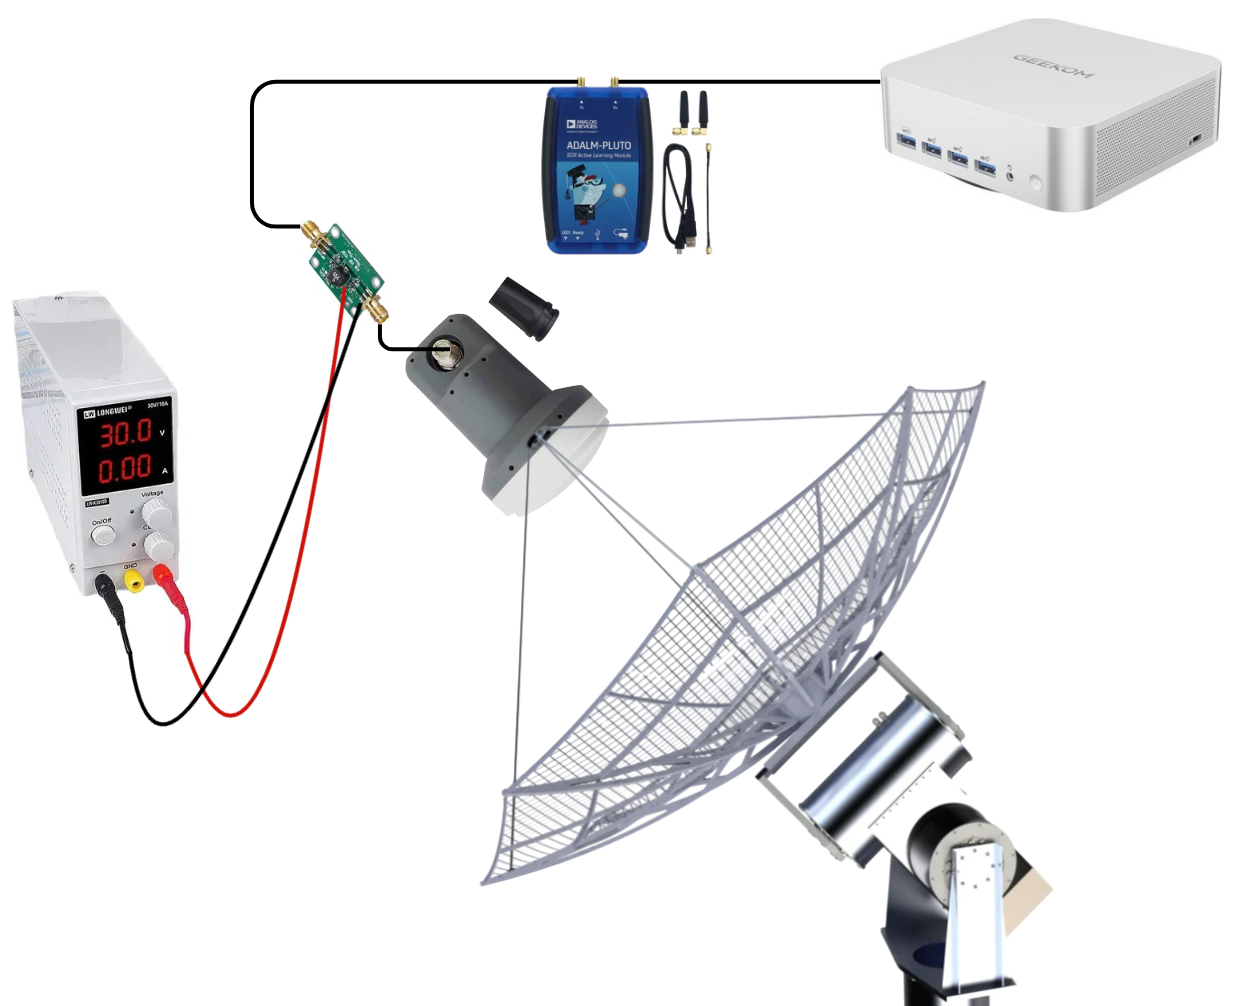
\includegraphics[width=0.7\textwidth]{figures/Inkscape/setup.png}
    \caption{Experimental hardware setup configured for the QO-100 geostationary satellite reception test.}
    \label{fig:qo100_hardware_setup_photo}
\end{figure}

Downstream in the transmission line, the \(\mathsf{IF}\)-modulated signal intercepted by the coaxial cable passes through a bias tee or \(\mathsf{Bias\text{-}T}\). This device acts as a direct current (DC) and RF diplexer, allowing the necessary supply voltage to be injected to activate the \(\mathsf{LNB}\)'s active circuits through the coaxial cable core itself, while simultaneously isolating the high-frequency signal component to protect subsequent stages. Subsequently, the filtered analog stream enters the software-defined radio or \(\mathsf{SDR}\), which is responsible for performing complementary analog filtering, automatic gain control, and analog-to-digital conversion (\(\mathsf{ADC}\)) to generate the in-phase and quadrature (\(\mathsf{I/Q}\)) digital samples. Finally, these digitized samples are transmitted via a high-speed \(\mathsf{USB}\) bus interface to the host computer (\(\mathsf{Computer}\)), where the previously analyzed digital signal processing, frame synchronization, and channel decoding pipeline is executed in real time.

\section{The Es'hail-2 Satellite and Multimedia Beacon} \label{sec:qo100_satellite}

To physically validate the RF front-end architecture described in the previous section, live satellite reception tests were required. Currently, the 2.4-meter ground station antenna lacks an active mechanical tracking system, rendering the capture of fast-moving Low Earth Orbit (LEO) satellites operationally unfeasible for the time being. To circumvent this physical limitation, we targeted \href{https://amsat-dl.org/en/eshail-2-amsat-phase-4-a/}{Es'hail-2} (also known as QO-100), a geostationary satellite positioned statically at $26^{\circ}$ East. Because it remains fixed relative to the ground station, it serves as an ideal geometric target to verify the integrity of our hardware chain.

\begin{figure}[htbp]
    \centering
    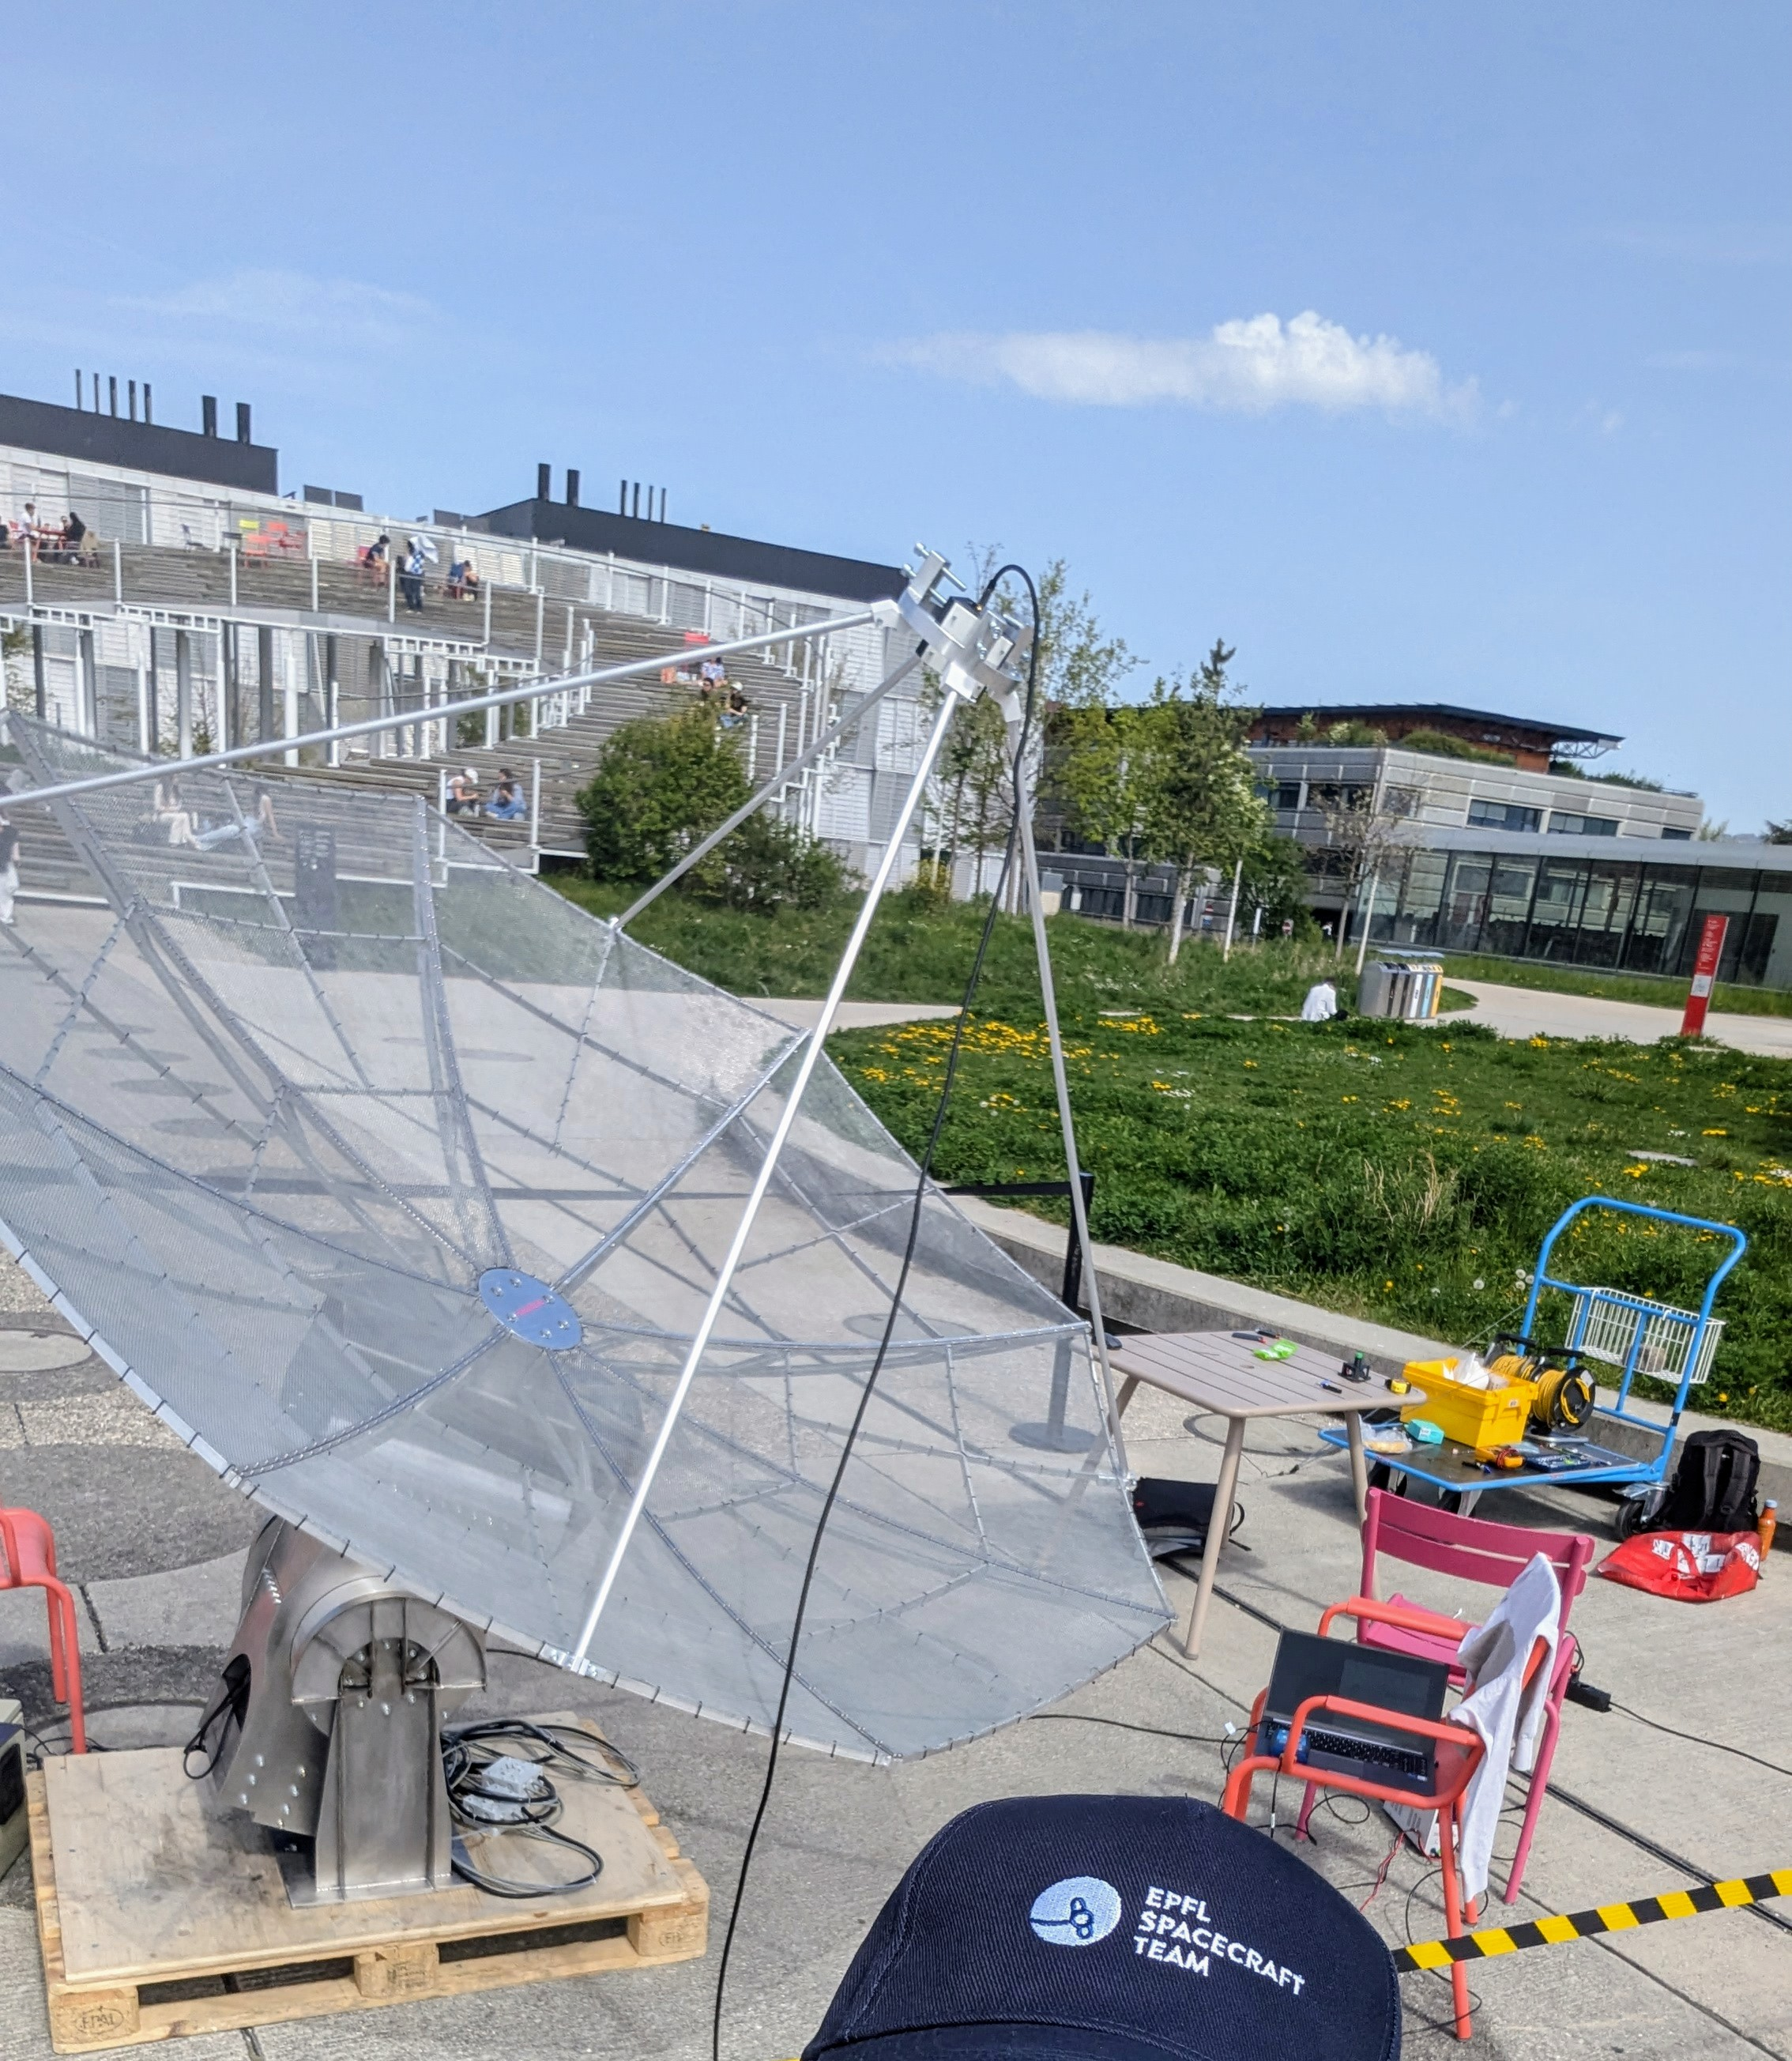
\includegraphics[width=0.7\textwidth]{figures/Inkscape/setup_photo.jpg}
    \caption{Hardware setup deployed for the QO-100 reception test, showcasing the SDR and the connected RF chain.}
    \label{fig:qo100_setup}
\end{figure}

Es'hail-2 hosts the first geostationary amateur radio transponder, developed by \href{https://amsat-dl.org/}{AMSAT-DL}. Specifically, the payload includes a \href{https://amsat-dl.org/en/p4-a-nb-transponder-bandplan-and-operating-guidelines/}{narrowband (NB) transponder} with a downlink spanning from $10489.550$ to $10489.800$~MHz. Within this band, the satellite continuously broadcasts a multimedia beacon. 

It is crucial to note that this multimedia beacon operates using the \href{https://dvb.org/?standard=second-generation-framing-structure-channel-coding-and-modulation-systems-for-broadcasting-interactive-services-news-gathering-and-other-broadband-satellite-applications-part-1-dvb-s2}{DVB-S2} (Digital Video Broadcasting - Satellite - Second Generation) standard, which relies on LDPC and BCH forward error correction. This contrasts fundamentally with the CCSDS (Reed-Solomon and Convolutional Coding) protocol developed throughout this project for the \textsf{CHESS} mission. Because the coding schemes are mutually incompatible, our custom GNU Radio receiver pipeline cannot be used to decode the QO-100 beacon. Consequently, this chapter serves as a valuable bonus milestone. Rather than testing our specific software demodulator blocks, it focuses on validating the physical hardware and the RF reception capabilities of the ground segment under real-world operating conditions. More importantly, it provides an ideal testbed to verify the execution of an alternative GNU Radio script in a live scenario, demonstrating the framework's capability to stream data, handle hardware interfaces, and perform complex baseband demodulation in real time.

\section{Hardware Validation and Demodulation Results} \label{sec:qo100_results}

The complete reception system was assembled and pointed towards the $26^{\circ}$ East orbital slot. The hardware setup, including the antenna feed, the SDR, and the data acquisition laptop, is depicted in \Cref{fig:qo100_setup}. 

Since our primary pipeline was strictly designed for CCSDS telemetry, we relied on the open-source community to perform the DVB-S2 software demodulation and validate our baseband I/Q samples. To achieve this, we utilized an existing, highly optimized GNU Radio flowgraph developed by Daniel Estévez \autocite{estevez_qo100_blog, estevez_qo100_gist}. His implementation handles the DVB-S2 physical layer framing, symbol synchronization, and LDPC decoding required to extract the payload.

\begin{figure}[htbp]
    \centering
    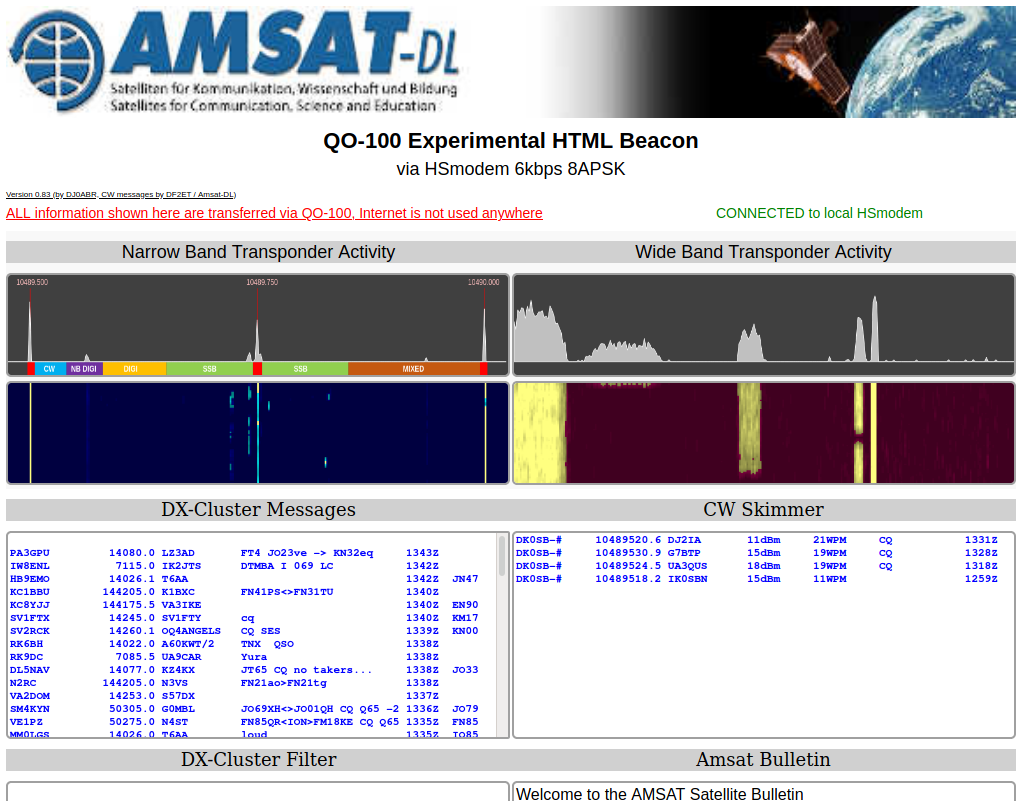
\includegraphics[width=0.95\textwidth]{figures/Inkscape/qo100_html.png}
    \caption{Demodulated HTML dashboard extracted from the QO-100 multimedia beacon, displaying live telemetry and transponder status.}
    \label{fig:qo100_html}
\end{figure}

The test was highly successful. The RF chain captured the X-band signal cleanly, and the third-party SDR flowgraph locked onto the beacon seamlessly. The resulting demodulated data stream from the DVB-S2 beacon consists of a periodically broadcasted HTML file. As shown in \Cref{fig:qo100_html}, this file renders a multimedia dashboard containing real-time satellite telemetry, transponder operational status, and AMSAT-DL bulletins. Successfully recovering this digital file provides definitive proof that the ground station's hardware architecture, from the parabolic reflector down to the USB bus, introduces minimal noise and operates perfectly within the required X-band specifications.